\chapter[General discussion]{General discussion}
\chaptermark{General discussion}
\label{cha:Chapter7}
\newpage

\section{Introduction}
The incidence of adverse health effects due to chronic undernourishment and micronutrient deficiencies are substantially higher in sub-Saharan Africa (SSA) compared to the rest of the world (\citealp{Godecke2018}). The individual and societal implications of this food insecurity are borne disproportionately by the rural SSA population (\citealp{Green2016}). Rural landholders are both vulnerable to the health burdens that stem from food insecurity, and central to improving the availability and affordability of a diversity of wholesome foods. To combat malnutrition, the global community needs to understand the interactions between food and nutrition (in)security and rural livelihoods. This understanding is currently missing.

The present understanding of food (in)security and rural livelihoods has been limited by the geographical and temporal scope of research efforts, and a lack of standardised rural household surveys. There is no one organisation with the resources to frequently monitor the vast diversity of rural communities at risk of food insecurity. Rather, rural household surveys are conducted nationally at in-frequent intervals and sub-nationally by a plethora of organisations. There have been considerable efforts to develop standardised rural household surveys over the past decade (e.g. \citealp{Carletto2009, Herrero2007}). However, these attempts to provide standardised survey designs have not resulted in substantial harmonisation and collaboration. \citet[p.~39]{Carletto2013} suggest that further harmonisation can be developed over time, with a ``combination of short-term fixes and long-term methodological advancements''. Recently, time-efficient proxies to food and nutrition security status have been developed -- marking a substantial methodological advancement (\citealp{Pisa2017, Keyzer2015}). These proxies can be readily incorporated into rural household surveys, providing comparable metrics across a diversity of studies to generate insights into the prevalence, spatial distribution and associations of food (in)security.

A growing body of literature utilising these food and nutrition security proxies has generated insights into the role that agricultural production and off-farm income plays in improving food and nutrition security. These findings, however, are dependent on the time of year that the survey is implemented and, have had a limited geographical scope -- limiting cross-site comparisons and more generalisable inference.

The primary objective of this thesis was to characterise food and nutrition security in rural landholding households in predominantly mixed crop-livestock agricultural systems of sub-Saharan Africa (SSA). Characterisation in this respect refers to describing the multiple facets of food and nutrition security, and identifying their associations with livelihoods. The secondary objective was to improve the methodological basis of household level food security studies.

This chapter first presents the research findings related to the harmonisation of rural household surveys to measure and monitor food and nutrition security. Harmonisation of rural household surveys is then discussed in terms of further methodological advances. A synthesis of findings related to food security and livelihoods is then provided. The discussion then continues with a focus on food and nutrition security in rural SSA in the context of nutrition-specific and nutrition-sensitive interventions; the stability of food and nutrition security throughout the year and; women's empowerment. The discussion then identifies further methodological advances for measuring food and nutrition security. This chapter is then concluded with a synthesis of findings.

\section{Harmonising rural household surveys}
\subsection{A balance between customisation and harmonisation}
A standardised rural household survey with an appeal to a wide user base was not available at the start of this PhD research. In a related PhD project, the rural household multi-indicator survey (RHOMIS) tool was developed to ``give a rapid, comprehensive overview of the farming system, which can be used to identify hotspot issues and to develop an evidence base to target deeper research'' (\citealp[P.~84]{Hammond2018}). Chapter 2 summarises this RHOMIS tool -- which was designed to collect a core set of modules, while being time-efficient, utilitarian, user-friendly, flexible and reliable (left-hand-side of Figure \ref{fig:07_1}). By being time-efficient, RHOMIS aims to minimise respondent fatigue and reduces the amount of time needed for survey design, implementation and analysis. The duration of the core set of modules in RHOMIS (listed in Figure \ref{fig:07_1}; provided in appendix 1 of \citealp{Hammond2018}) is estimated to be between 40 to 60 minutes (Table \ref{tab:02_1}). The duration of RHOMIS is half that of comparable surveys -- such as the `integrated modelling platform for mixed animal crop systems' (IMPACTlite; compared in Table \ref{tab:03_1}). The food availability indicator took the most time to collect, at a maximum of 35 minutes, followed by diet diversity, taking 10 minutes. The ease of enumeration was evaluated favourably for each module, with over 50\% of interviews being perceived as `easy' by the interviewer (Chapter 2).

The utilitarian design of RHOMIS means that every question is asked for a purpose. While this may sound logical, it is the norm in non-standardised household surveys to ask additional questions -- just in case they are important. In RHOMIS, each question is either incorporated into a composite indicator or used directly. If a variable or module proves to be ineffective, then it is revised or removed. The user-friendly principle of RHOMIS is most prominent in the design of the computer-aided personal interview (CAPI) system, which reduces the need for paper-and-pen entry. These design principles reduce survey time and respondent fatigue and provide efficiencies in data entry and data analysis.

The principle of flexibility refers to the extendibility and localisation of the survey. The core and additional modules are listed in Figure \ref{fig:07_1}, providing potential extensions into water, sanitation and hygiene (WASH), household expenditure and many more aspects of rural livelihoods. A survey needs to be adapted to the local language, units (standard measures of volume), foods and species. Over time, these localisations can be reused and improved upon. The RHOMIS tool is now available in 9 languages and has been localised to 48 sub-national locations in SSA, South-East Asia and South and Central America.

The credibility and consistency of data collected using RHOMIS was evaluated in Chapter 3. RHOMIS stayed within credible bounds more frequently than IMPACTlite and the Living Standards Measurement Study -- Integrated Survey on Agriculture (LSMS-ISA). The positive performance of RHOMIS in this respect could be attributed to the localisation of units -- minimising respondent estimation error. The inconsistency between IMPACTlite and RHOMIS (forming a test-retest study) was most evident in the diet diversity indicator. The limitations in dietary data collected in IMPACTlite may be explained by an unfortunate combination of poor question design and excessive survey duration. In contrast, the targeted questions in RHOMIS resulted in more realistic diet diversity estimates as there was less item non-response for commonly consumed food groups such as cereals and beans.

The design of RHOMIS has appealed to a diversity of users, including researchers and development organisations. The users of RHOMIS has evolved into a community of practice over the course of this PhD research. The RHOMIS community of practice has made substantial progress in harmonising data collection activities (www.rhomis.org). Throughout the duration of this PhD, the harmonisation of sampling, data pre-processing and testing of proxies was managed on a case-by-case basis (methodological developments listed in the top right of Figure \ref{fig:07_1}). These studies served as a proof of concept of effective rural household survey harmonisation. Now that there is an engaged community of practice, there are opportunities to make further methodological advances -- including introducing sampling guidelines, providing additional modules to validate indicators and introducing alternative modes of data collection (bottom right of Figure \ref{fig:07_1}). This section discusses each of these potential methodological advances.


\subsection{Further methodological advances for the RHOMIS approach}

\textit{Sampling support} was provided to organisations that did not have access to this support elsewhere. Rigorous sampling
is the basis of generalisable inference. All datasets utilised in Chapters 4 to 6 impliment multi-stage clustered sampling. Chapter 4 is based on geographically random sampling across villages within a 10-by-10 kilometre research area. Chapter 5 is based on purposively selected villages with random sampling from lists of households. Chapter 6 is based on several independent studies, sampling from lists of households within villages, but differing geographical bounds (e.g. Nationally representative and within a 10-by-10 km area). The consistency of sampling can be improved by providing \textit{sampling guidelines} that provide details on sample size determination (including reliability assessments -- Chapter 3) and various sampling methods (e.g. geographically random). The sampling method employed and suitable weightings would then be incorporated in the RHOMIS \textit{database} as \textit{meta-data}. This \textit{meta-data} would then allow the pooling of data-sets with similar sampling methods and geographical bounds.

There are also opportunities to critically assess the \textit{proxies} used in RHOMIS by \textit{validation} against more accurate methods. Specifically, in any given study, more detailed data can be gathered from a smaller subset of households to compare with the coarser measurement (referred to as `two-method measurement designs', \citealp{Little2013}). Validating proxies as well as meeting the primary research objectives is challenging to implement. It is particularly challenging to develop and implement two experimental designs -- one for the primary purpose of the research and another for the validation study. In the RHOMIS tool -- where much of the uncertainty of experimental design has been standardised -- an additional validation study is more tractable. Candidate variables for this process include: land size, diets, localisation units, crop yields and milk yield. By implementing two-method measurement designs, there is the potential to correct for errors in the broader dataset and identify methodological improvements.

\begin{figure}
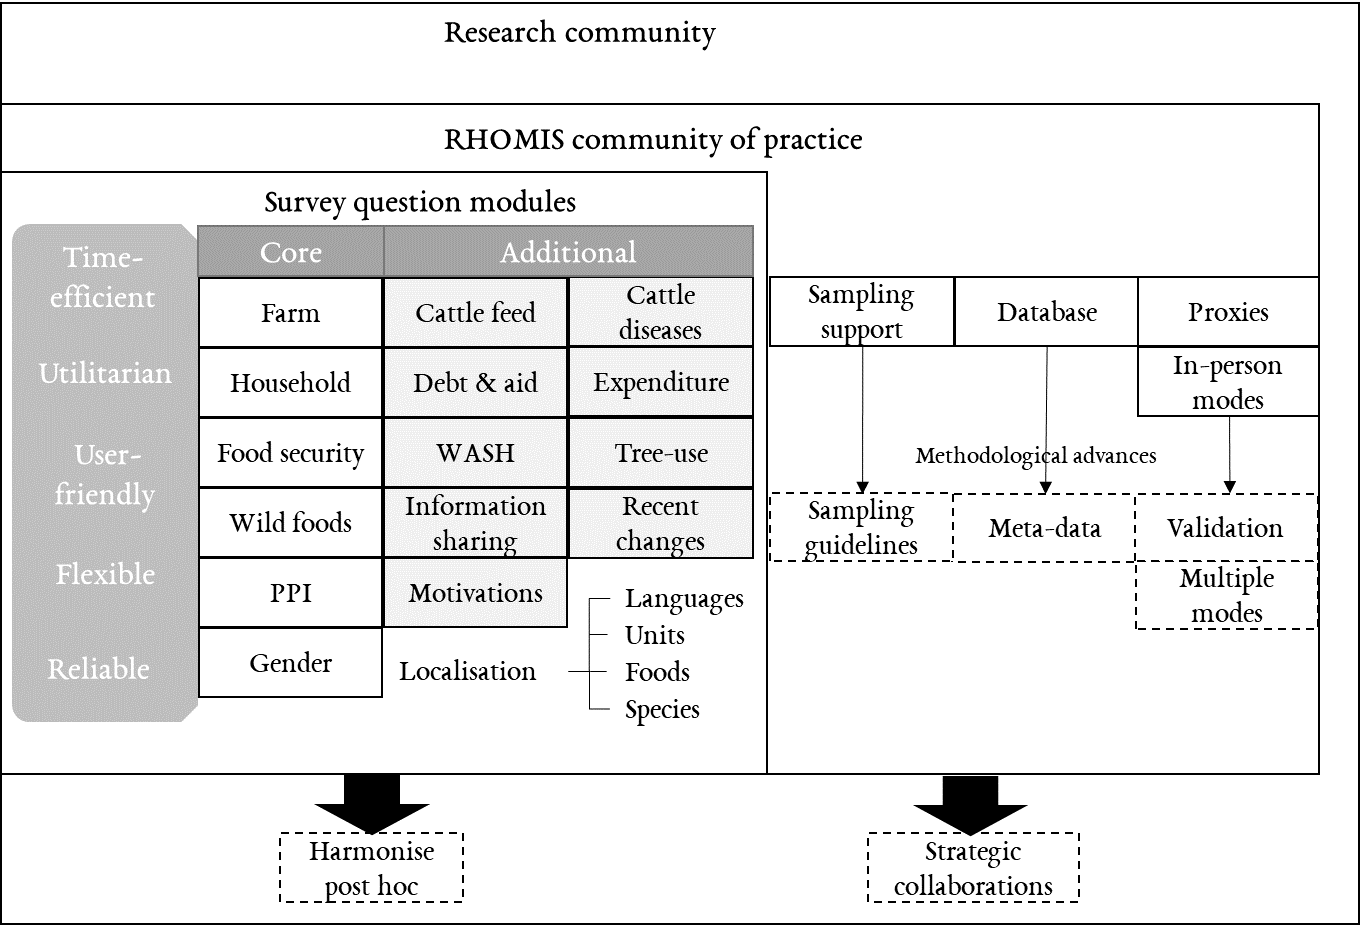
\includegraphics[width=1\textwidth]{figs_07/RHOMIS.png}
  \captionsetup{singlelinecheck = false, justification=justified} %left justify caption
  \caption{Summary of progress and pending developments to harmonise rural household surveys. Including the progress out of poverty index (PPI) and; water, sanitation and health (WASH) modules from the rural household multi-indicator survey}
  \label{fig:07_1}
\end{figure}

Research can also be explicitly carried out to validate indicators. In this instance, an experiment is designed to compare alternative indicators against a `gold standard'. An example of this would be to compare the modified household diet diversity recall periods (Chapters 5 and 6) to quarterly 24-hour dietary recall (24hR). Such a research effort could validate one of the alternatives, and potentially identify modifications that need to be made.

The RHOMIS tool has relied on \textit{in-person modes} of data collection with multiple recall periods. The reliance on multiple recall periods means that respondents may need to remember a set of circumstances from up to 11 months prior in order to answer a question -- having a negative impact on measurement precision (\citealp{Beegle2012}). In an initiative such as the RHOMIS community of practice, it is not possible to force users to revisit households multiple times throughout the year. Relying on recall has been a pragmatic reality.

As an alternative to multiple recall periods, \textit{multiple modes} of data collection can be used to build relationships with respondents in-person and then to follow-up with the same respondents in a cost effective manner. In particular, as 46\% of the SSA population is now connected to mobile networks there is the potential to engage rural households through the use of mobile phones (\citealp{GSMAIntelligence2016}). Short messaging services (SMS) and computer-assisted telephone interviewing (CATI) are two alternatives in this respect. In a comparison between face-to-face interviews (CAPI) and CATI, Lamanna et al. (accepted) found that telephone interviews were effective for the majority of questions asked. Sensitive questions on child and maternal health differed significantly by mode. There were also some mode effects at the food category level, with pulses reported more frequently in CATI and milk reported less frequently. These findings suggest that data collection through CATI can introduce biases. The cost of CATI interviews were reported to be US\$5 per successful survey, compared to US\$16 for face-to-face. One concern raised by Lamanna et al. (accepted) was that CATI may disproportionately exclude those less likely to have access to a mobile phone, such as the less wealthy and young women. Aside from the cost savings, this method has the potential to reduce recall period, and to improve the monitoring of communities in conflict zones (as in northern Yatenga -- Chapter 5) or communities that are geographically inaccessible.

In addition to methodological improvements, there are also opportunities to \textit{harmonise} RHOMIS data with other research efforts and to form strategic collaborations (bottom of Figure \ref{fig:07_1}). To-date, RHOMIS has been harmonised with other datasets, increasing the total number of observations from 25,000 to 50,000. Even with such a large database, there are still geographical and temporal gaps which can be addressed by forming \textit{strategic collaborations}, to harmonise with existing RHOMIS data. This can work by coordinating with specific organisations (e.g. UNICEF, CARE or World Vision) that are delivering projects in food insecure locations that currently lack harmonised data.

The harmonisation of rural household surveys is the result of more than a decade of steady progress. Rural households can now be characterised in a standardised way, enumerating multiple indicators of food and nutrition security. These indicators include: food availability, food security of access, diet diversity, food-self-sufficiency (adequacy ratios), sources of micronutrients and duration of food scarcity. This thesis draws on a total of 8,257 household interviews, conducted in 14 projects to characterise food and nutrition security in rural landholding households.

\section{Food and nutrition security in SSA}
\subsection{Prevalence and spatial heterogeneity of food insecurity}
In the sample of rural landholders across SSA, as many as 40\% of households were classified as severely food insecure in the `lean' period -- defined as the period of food scarcity. In general, households sourced two food categories on a daily basis in the `lean' period and three food categories in the `flush' period (median; results not shown). The implications of diet diversity on micronutrient deficiencies (hidden hunger) differed depending on which food categories were sourced. Disaggregating the count of diet diversity, it was reported in Chapter 6 that 68\% of households did not have a year-round daily source of calcium, 38\% lacked a daily source of iron, 37\% lacked a daily source of thiamine (vitamin B1), 51\% lacked a daily source of riboflavin (vitamin B2), 44\% lacked a daily source of niacin (Vitamin B3), 35\% lacked a daily source of pyridoxine (vitamin B6) and 65\% lacked a daily source of cobalamin (vitamin B12) (Table \ref{tab:06_2}). The prevalence of chronic and hidden hunger was highly variable between and within regions. Within-region variability is evident in Chapter 5, where households in two relatively similar provinces of Burkina Faso exhibited markedly different rates of food insecurity. More generally, instances of food insecurity differed by household composition, farm-business characteristics, income diversification and agro-ecological zone (AEZ; Chapter 6).

\subsection{Food and nutrition security and livelihoods}
Household composition was significantly associated with food security across sampled regions of rural SSA (Chapter 6). Female-headed households were more likely to be chronically hungry in the lean period and to lack sources of calcium -- where the head of the household is defined by asking in the initial stages of the interview. It was also the case that lower performing `subsisting' households identified in Chapter 4 were predominantly female-headed. Similarly, households with children under the age of 10 were more likely to be chronically hungry in the lean period, and more likely to lack sources of calcium (Table \ref{tab:06_3}). Households with children under the age of 10 tended to have more inhabitants, the same level of income, lower progress out of poverty and therefore higher instances of hunger (Appendix Table \ref{tab:C_14}). These findings support the need for programmatic strategies on gender inclusion (bottom right of Figure \ref{fig:07_3}; \citealp{Mason2015}), as well as the need for focusing on maternal and child nutrition (\citealp{Sharma2017, DePee2017, Arimond2004}). A livelihood in this thesis is defined as the way resources are utilised to maintain the wellbeing of an individual or social group (\citealp{Blaikie1994}). In Chapter 4, substantial changes in livelihoods were observed over three years -- suggesting that livelihoods are dynamic over a short period of time. Livelihoods were also observed to be highly variable (Chapters 4, 5 and 6). For example, Table \ref{tab:05_2} summarises two sites with relatively low production potential; within and between these sites there was substantial variation in household inhabitants, land area and livestock holdings. Despite this variability, several livelihood characteristics were identified to be associated with food security across sampled regions of SSA -- including size of land area, size of livestock holdings, production diversity, level of gross income and extent of income diversification -- i.e. earning off-farm income.

Households with larger land area cultivated were more likely to have more diverse diets. The effect of land cultivated on diet diversity was most substantial in the flush period. As livestock holdings increased, households were more likely to have access to sources of all micronutrients -- regardless of AEZ. The diversity of livestock products produced by a household, furthermore, was positively associated with food security of access, diet diversity in the lean period as well as being positively associated with calcium, iron, thiamine, niacin, vitamin B6 and vitamin B12 (Chapter 6). Crop production diversity was positively associated with food security of access and diet diversity regardless of AEZ. However, the association between crop production diversity and accessing sources of micronutrients differed by AEZ. Households in humid and sub-humid zones were more likely to access micronutrient sources as crop production diversity increased.

In reality, it is the combination of these livelihood characteristics that influences food security status. Chapter 6 identifies four distinct farm types, labelled: `Specialised cropping', `Diverse cropping', `Specialised cropping and livestock', and `Diverse cropping and livestock'. The prevalence of severe food insecurity and gaps in micronutrient sources depended on farm type. In humid and sub-humid AEZs, households with diverse crops had a lower prevalence of severe food insecurity. Additionally, `Diverse cropping \& livestock' households in humid and sub-humid zones had a lower prevalence of gaps in all micronutrients. In semi-arid zones, the difference between farm types was more distinct, where households with a livestock component to their farm had a lower prevalence of severe food insecurity and gaps in all micronutrients.

In this discussion, the higher performing farm types that keep livestock are further disaggregated by land area cultivated (Figure \ref{fig:07_2}). In humid and sub-humid zones, households labelled as `Diverse cropping medium-large' (n = 493) were less likely to be chronicly hungry and were more likely to have access to sources of calcium and niacin compared to their smallholder counterparts (n= 797; mixed-effects logistic regressions; 95\% CI < 0, Appendix Table \ref{tab:C_15}). In semi-arid zones, `Specialised cropping medium-large' (n = 402) were less likely to be chronicly hungry and were more likely to have access to sources of iron, thiamine, riboflavin, niacin and pyridoxine when compared to their smallholder counterparts (n = 343; mixed-effects logistic regressions; 95\% CI < 0; Appendix Table \ref{tab:C_16}). These results suggest that all the relevant interactions between livelihood characteristics are not fully captured in the modelling of Chapters 5 and 6. Rather, food security status is determined by the combination of land area, livestock holdings, production composition and land area -- differing by AEZ.

\begin{figure}[H]
\includegraphics[width=1\textwidth]{figs_07/prevalence_weighted2.png}
  \captionsetup{singlelinecheck = false, justification=justified} %left justify caption
  \caption{Proportion of livestock keeping households (n = 4,028 weighted by population) chronically hungry or lacking micronutrient `source' by farm type, scale and agroecological zone. A 95\% confidence interval is represented by vertical lines}
  \label{fig:07_2}
  \small

\end{figure}

Income diversification was also found to be associated with food security. In Chapter 4, households in Lushoto earning off-farm income in the `Rising high-value crops' cluster had significantly higher diet diversity in the flush period when compared to others in the cluster. In Chapter 5, households in northern Burkina Faso that earned off-farm income were less likely to be severely food insecure. Off-farm income had a significantly positive effect on diet diversity in Seno province as gross farm income increased. However, in Yatenga province, it was predicted that households not earning off-farm income had a greater potential to have more diverse diets. More generally across a diversity of rural communities of SSA, Chapter 6 showed that off-farm income was positively associated with food security of access, diet diversity, as well as calcium, riboflavin and vitamin B12. The difference between Chapter 5 and 6 in this respect suggests that off-farm income is positively associated with improved food security status in general, but can have differing effects at a site disaggregated level.

The associations between livelihoods and food security are mediated by food sourcing decisions. Households can access food from their own farm, through purchases or by trading, hunting or gathering. This thesis focused on two channels of food access, from own-farm production and purchased foods (presented as `own production' and `income' channels in Figure \ref{fig:07_3}). In northern Burkina Faso, own-farm sourcing had the potential to fulfil much of the household's energy needs, and the diversity of diets was most differentiated through purchased foods (Chapter 5). However, in an analysis of multiple sites across SSA, Chapter 6 demonstrates that households fail to purchase food categories that nutritionally complement their own agricultural production. This means that less production diverse households are less likely to access sources of specific micronutrients, such as calcium (dairy), vitamin A (vitamin A rich fruits and vegetables) and vitamin C (other fruits).

Multiple statistically significant associations were identified in this thesis. The causality of these associations could not be fully represented in the models of Chapters 5 and 6. For instance, household composition is associated with food security because headship and stage of life influence livelihood characteristics -- not due to a direct causal association. Several livelihood characteristics were associated with food security. It is the combination of these livelihood characteristics and agro-ecological production potential that drive the availability of food and income. Food security is then mediated by food sourcing decisions related to own-farm food availability and income availability. While purchases tend to drive overall diet diversity, a few select food categories are more readily sourced if available through the own-farm channel. These findings suggest that improving food security through rural livelihoods requires a focus on increasing supply, adding nutritional value through the own-farm channel and increasing demand for nutritious foods (relating to the three strategies of Figure \ref{fig:07_3}).

\section{Interventions, stability of food security and gender}
\subsection{Maximising the nutritional impact of interventions}
It has been estimated that much of the chronic and hidden hunger quantified in this thesis can be alleviated by implementing a set of \textit{nutrition-specific} interventions at a cost of US\$9.6 billion per annum -- including programs on fortification, micronutrient supplementation and exclusive breastfeeding promotion (\citealp{Bhutta2013}). It is emphasised in \citet[p.~452]{Bhutta2013} that if such expenditure is ``linked to \textit{nutrition-sensitive} approaches--i.e., women's empowerment, agriculture, food systems, education, employment, social protection, and safety nets--they can greatly accelerate progress in countries with the highest burden of maternal and child undernutrition and mortality.''. The implementation of \textit{nutrition-specific} interventions, in combination with \textit{nutrition-sensitive} interventions, calls for greater coordination between intervening agencies working across multiple disciplines.

The International Fund for Agricultural Development (IFAD) framework on nutrition-sensitive value-chains defines three strategies that encompass \textit{nutrition-sensitive} agricultural, food systems and education interventions -- namely, \textit{increase supply}, \textit{increase demand} and \textit{add nutritional value} (\citealp{DeLaPena2018}). Strategies to \textit{increase supply} (\citealp{Ruel2013}) aim to increase farm, regional and national food supply by improving productivity and reducing waste (top left box of Figure \ref{fig:07_3}). Strategies that \textit{increase demand} for nutritious food aim at product and nutritional education (bottom-left of Figure \ref{fig:07_3}). Strategies that \textit{add nutritional value} aim to improve the nutritional content of food produced, for example, by promoting vitamin A rich sweet potato; maintain the nutritive quality, for example through grain storage or refrigeration; and, \textit{improve food safety}, for example by reducing aflatoxin contamination. Several \textit{nutrition-specific} interventions also add nutritional value to the food system and so fall within the scope of the IFAD framework. The remainder of this subsection discusses \textit{increasing supply} and \textit{adding nutritional value}.

The framework acknowledges that \textit{increasing supply} and incomes will not directly improve nutritional status. Rather, individuals need to decide how the additional supply is to be utilised (`own-farm channel') and how income is to be spent (`income channel' in Figure \ref{fig:07_3}; \citealp{Price2018, Kazianga2017, Galie2015}). In fact, a concern of agencies implementing agricultural interventions is that the economics of productivity gains will drive increased specialisation and market orientation, which would reduce production diversity and compromise nutritional status (\citealp{Tscharntke2012}).


\begin{figure}[H]
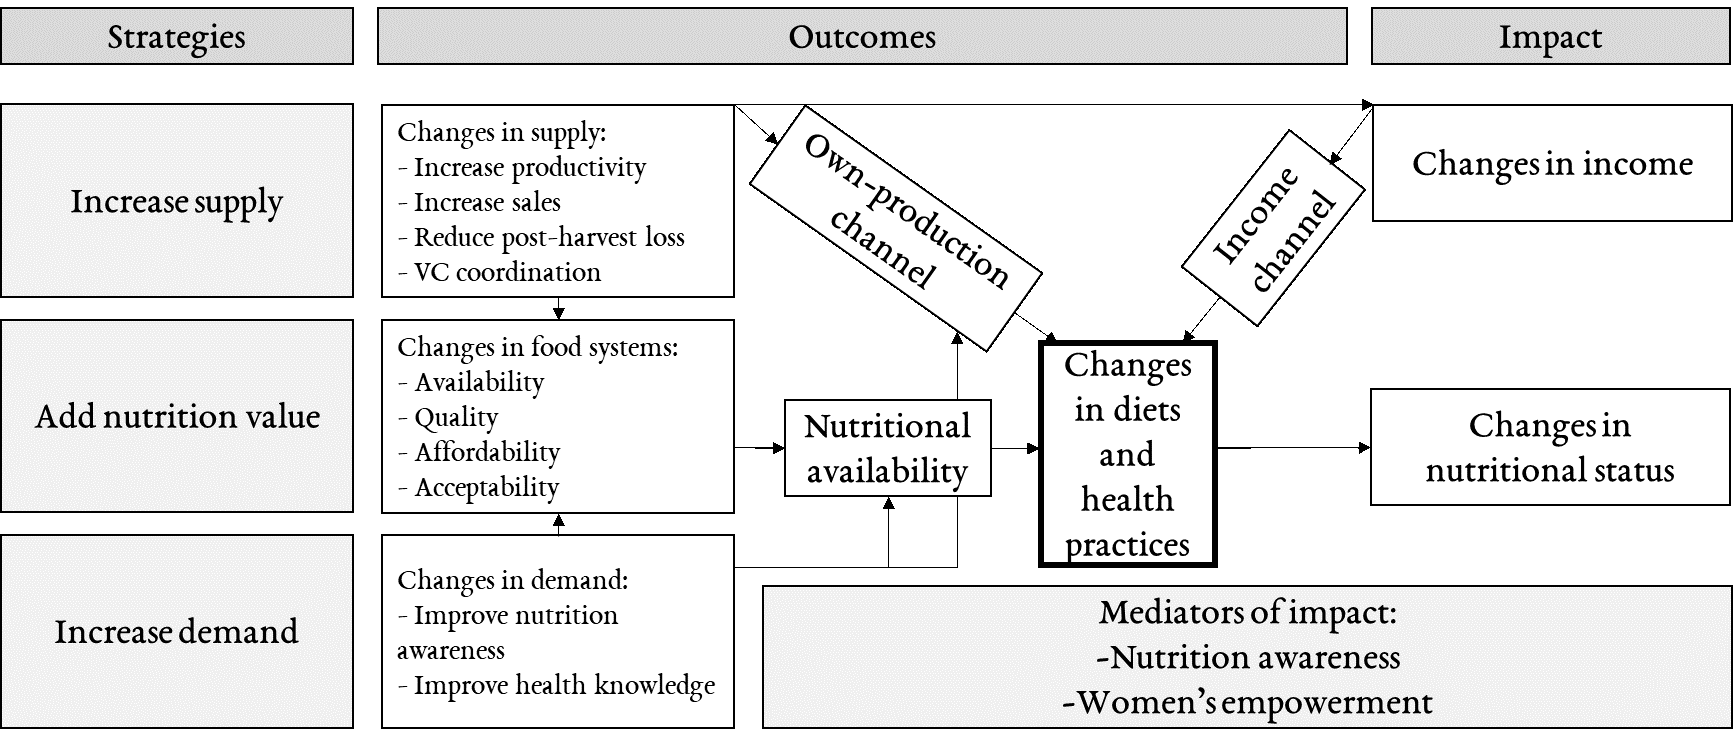
\includegraphics[width=1\textwidth]{figs_07/IFAD_frameworkv2.png}
  \captionsetup{singlelinecheck = false, justification=justified} %left justify caption
  \caption{Impact pathways of food system-based nutrition-specific and nutrition-sensitive interventions}
  \label{fig:07_3}
  %\small
  %\raggedright
  \vspace*{-3mm}
  \caption*{VC = value-chain \\
 	(Reproduced with permission from IFAD, 2018)}
\end{figure}



The literature indicates that there are several options for \textit{adding nutritional value} to food systems. Evidence suggests that interventions supporting livestock production can significantly reduce micronutrient deficiencies and health outcomes. For example, horticulture and poultry training has been found to increase vitamin A levels (\citealp{Masters2018}). Specifically, increasing animal-source food consumption has been found to significantly reduce stunting in low and middle-income countries (\citealp{Headey2018}).

The breeding and genetic modification of crops has also been a promising avenue to add nutritional value to food systems -- referred to as biofortification. Biofortification of pro-vitamin A crops (orange flesh sweet potato and maize; \citealp{Bouis2017}) and iron (beans and pearl millet) have been found to be effective physiologically and economically (\citealp{Osendarp2018}). For example, it has been estimated that interventions supporting sweet potato cultivation can save one disability average life year (DALY) for the cost of US\$15 -20 -- where a DALY is a standardised measure of human health and life expectancy (\citealp{Osendarp2018}). The biofortification of folate (B9) has also been tested in several crops and combined B vitamin biofortification is being explored (\citealp{Strobbe2018}).

Directly adding micronutrients to food systems has been identified as being one of the most cost-effective means of addressing hidden hunger (\citealp{Bhutta2013, Osendarp2018}). Referred to as fortification, this process adds specific micronutrients at safe levels to commonly consumed foods -- such as iodine to salt and bread, zinc and B vitamins to processed cereals, and vitamin D to foods with high oil content. Fortification is most commonly and cost-effectively implemented in collaboration with large-scale food processors. However, such processed foods may not be available to those at most risk to hidden hunger. In these instances, own-produced foods can be fortified by adding micronutrient powders -- referred to as complementary food production. Such complementary food production interventions-- have been effective at increasing iron and zinc intake in Ethiopia and Nigeria (\citealp{Masters2018}).

The implementation of agricultural-based interventions to \textit{add nutritional value}, however, is not as straightforward as fortification programs. As an example, \citet{Jenkins2018} identified a wide range of factors constraining adoption of orange flesh sweet potato in Mozambique -- including: taste preferences, availability of seed, and volatility of markets. To overcome the challenge of low adoption, programs can be designed as `packages', which combine agricultural and non-agricultural interventions, such as biofortified crops, complementary feeding, social safety-nets and women's empowerment (\citealp{Ruel2018, Jaenicke2013}). The micronutrient disaggregated analysis in Chapter 6 allows for the identification of potential dietary gaps of sub-populations, facilitating the targeting of such intervention packages. This packaging of interventions, however, requires greater collaboration between intervening agencies working across multiple disciplines, which is currently lacking.

There are several mediators to the effectiveness of nutrition-specific and nutrition-sensitive interventions. The following subsections discuss two mediators raised in this thesis, namely: the temporal variability of food and nutrition security, and the empowerment of women.

\subsection{Stability of food and nutrition security throughout the year}
The long-term stability of food and nutritional security is the ultimate goal of any effort to address chronic and hidden hunger. To support long-term stability, providing social protection and safety-nets have been identified as important \textit{nutrition-sensitive} interventions (\citealp{Bhutta2013}). An underlying challenge is that livelihoods are influenced by seasonal factors which determine the duration of scarcity, which tend to differ between and within AEZ. Figure \ref{fig:07_4} presents the variability in duration of food scarcity in Burkina Faso and Kenya, by AEZ.

In Burkina Faso, where the majority of households are located in semi-arid zones, over one-third of households experienced food scarcity in August (Figure \ref{fig:07_4}). In semi-arid zones of Burkina Faso, 63\% of households experienced between one and three months of food scarcity. In contrast, 48\% of households in humid and sub-humid zones did not experience any food scarcity months. The pattern of food scarcity months differed in Kenya, with households in semi-arid zones experiencing longer durations (2-6 months), later in the year (September-October) and households in humid and sub-humid zones experiencing shorter durations (2-4 months) earlier in the year (April). In the context of climate change and globalised markets, rural livelihoods are more exposed to climatic and market shocks, exposing households to the risk of more severe and longer food insecure periods (\citealp{Fanzo2018}).


\begin{figure}[H]
  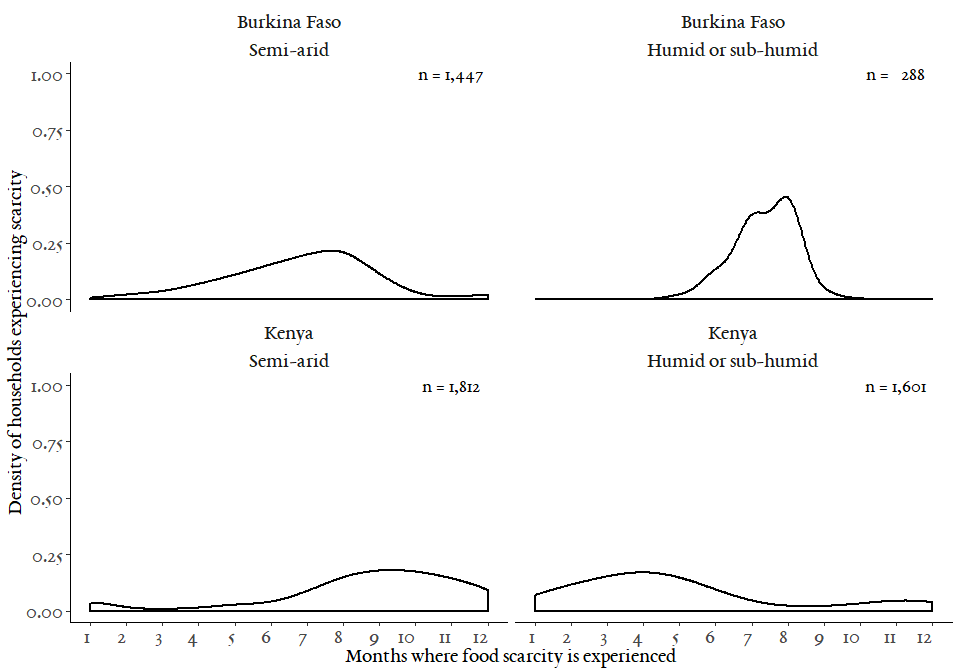
\includegraphics[width=1\textwidth]{figs_07/ScarceMonths_2.png}
  \captionsetup{singlelinecheck = false, justification=justified} %left justify caption
  \caption{Food scarcity months (January to December) of sampled households in Burkina Faso (n = 1070) and Kenya (n = 1030) sample by AEZ}
  \label{fig:07_4}
  %\small
  %\raggedright
  \vspace*{-3mm}
 	\caption*{(Observations from Chapter 6 only)}
\end{figure}

Increased exposure to climatic and market shocks have direct implications for the stability of food and nutrition security (\citealp{Ruel2018, Tomich2018, Jaenicke2013, Hussein1998}). Chapter 4 provides a case-study of households rapidly changing their climatic and market risk exposure. In Lushoto, Tanzania, households were found to be dynamic, making substantial changes to their farm over the course of three years. There appeared to be different approaches to market and climatic risks between the two higher performing clusters of households. The first cluster of households cultivated more land, with a portfolio of coffee, tomatoes, market vegetables, staples as well as keeping livestock species (agrobiodiverse production); the second cluster of households focused on livestock and staple crops. These differing production compositions have implications for risk exposure. Households in the first cluster may be less resilient to shocks in labour availability (e.g. due to ill health). Households in the second cluster may be more exposed to climatic and market risks due to a reliance on a limited range of crops and the absence of livestock. Notably, social safety-nets in the region have changed considerably over the past 30 years, where ``Access to unimproved subsistence land ... was still accepted as every resident's right... right up until the end of 1988'' (\citealp[p.~183]{Feierman1990}), and now safety-nets are based on family and social networks.

The role of agrobiodiversity (count of species) in the long-term stability of food and nutritional security was discussed in Chapter 5. While production diversity has a logical link with micronutrient sufficiency, the direct association with agrobiodiversity was weak (see also \citealp{Berti2015}). Rather, agrobiodiversity can co-exist with a market orientated strategy and provide risk management functions (\citealp{Waha2018a, Jaenicke2013, Tscharntke2012}). Livestock keeping -- as part of a diversified portfolio -- provides soil health benefits through the recycling of nutrients, as well as reducing livelihood risk by being a means to store capital (\citealp{Moll2005, Slingerland2000}). Similarly, diversified crop production can contribute to pest and disease management; reduce the market risk of volatile prices, and; can also be a part of a soil health strategy (e.g. nitrogen fixation or cover cropping to reduce erosion; \citealp{Lin2011}). Each of these benefits can reduce the risk exposure of a livelihood, specifically in relation to environmental or economic shocks. The packaging of interventions, therefore, would be appealing to production and income diversified rural households -- where they can adopt the most suitable innovations for their livelihoods.

\subsection{Women's empowerment and food security}
Land management, practice adoption and food access decisions are mediated by intra-household dynamics (Stirling, et al., submitted; Tavenner et al., submitted; \citealp{Dzanku2019, Price2018, AnderssonDjurfeldt2018a, Haider2018, Kazianga2017, Galie2015}). The empowerment of women -- in particular -- has been found to be central in changing diets and improving nutritional status (Figure \ref{fig:07_3}; \citealp{Rao2018, Price2018, Jaenicke2013}). As an extension of the analysis in Chapter 6, Table \ref{tab:07_1} presents a summary of households by gender of household head. In line with \citet{AnderssonDjurfeldt2018a}, these extended results suggest that there was a significant asset bias against female-headed households -- cultivating less land and owning fewer heads of cattle (Table \ref{tab:07_1}). Female-headed households exhibited a similar level of market participation to their male-headed counterparts. Despite this negative asset bias, female-headed households have comparable energy adequacy ratios from own-farm consumption, duration of scarcity and diet diversity in the lean period -- when compared to male-headed households (Table \ref{tab:07_1}). Chronic hunger, however, was found to be associated with female headship (Table \ref{tab:06_3}).
These findings indicate that the prevailing asset biases are the central areas for concern -- whether they be cultural or financial.

\begin{table}[H]
  \captionsetup{singlelinecheck = false, justification=justified} %left justify caption
   \caption{
    Livelihood characteristics and food security status by head of household (median; n = 6,343)
  }
  \label{tab:07_1}
  \small
  \centering
  \begin{tabularx}{\textwidth}{@{}lYYl@{}}  %{p{2cm}p{3cm}p{3cm}p{3cm}p{3cm}}
    \toprule
        &  Female headed & Male headed & $\beta_{female}$ (SE)  \\ %multirow spreads content over 3cm
        &(n=5,270)&(n=1,073)& \\
    \midrule

Household inhabitants (adult eq) & 4.4 (3.3) & 5.7 (4.1) & -0.86 (0.12)*$^\psi$\\
Land cultivated (ha) & 1.21 (1.40) & 1.62 (2.40) & -0.70 (0.20)*$^\psi$\\
Large ruminants (number) & 0 (4) & 1 (7) & -3.49 (1.08)*$^\psi$\\
Market participation (\% kcal sold) & 18 (0.48) & 23 (0.50) & -0.02 (0.01)*$^\psi$\\
Gross income (PPP) & 217 (946) & 254 (1,312) & 0.07 (8.31)$^\psi$\\
Progress out of poverty index (0 - 100)${\dag}$ & 38 (26) & 39 (28) & -0.59 (0.51)$^\psi$\\
Energy adequacy ratio (kcal consumed adult eq requirements$^{-1}$) & 0.42 (0.76) & 0.48 (0.81) &	-1.41 (1.18)$^\psi$\\
Length of lean period &	3 (3) &	2 (3) &	0.01 (0.02)$^\psi$\\
Diet diversity in the lean period (sourcing weekly) & 2 (3) & 2 (3) & -0.04 (0.07)$^\varphi$\\
    \bottomrule
  \end{tabularx}
  \footnotesize
  \raggedright
  %\caption*{
*\textbar95\% \textbar Credible Interval > 0; described in Chapters 5 \& 6\\
$^\psi$Linear regression. Random effects from villages nested within projects, weighted by population\\
$^\varphi$Negative binomial regression. Random effects from villages nested within projects, weighted by population\\
$^{PPP}$Purchasing power parity. See methods section of Chapter 6\\
$^\dag$Defined in Chapters 2, 3, 4, 5 \& 6

\end{table}

The differences between male-headed and female-headed households demonstrate that gender is an important mediating factor in accessing productive assets and therefore in mediating food security status. It is also expected that the empowerment of women will have an influence on food security within male-headed households (\citealp{Dzanku2019, Price2018, AnderssonDjurfeldt2018a}). Studies related to this thesis have used the RHOMIS database to identify associations between the empowerment of women and practice adoption (Stirling et al., submitted), as well as the empowerment of women and market orientation (Tavenner et al., submitted). To explore the role of gender in mediating food security empirically, we first calculated a gender equity indicator, quantifying gender disaggregated labour allocation, decision-making, asset ownership and control of income (Chapter 2). This indicator was used in exploratory analysis but was not found to be associated with the various food security indicators. This gender equity indicator was then disaggregated into labour allocation, decision-making, ownership of assets and control of income. Again, these metrics were not found to be associated with food security indicators. However, just because this thesis did not identify associations between food security and gender within male headed households, it does not negate the importance of gender. Rather, it may be a limitation of the quantitative indicator or the analytical approach used in this thesis.

Quantifying complex social dynamics in a cross-sectional interview is challenging. This challenge is compounded by the diversity of surveyed communities. The formulation of questions on labour allocation, decision making, ownership of assets and control of income can be standardised in a protocol and through enumerator training. For example, a protocol may specify question phrasing, such as: ``How much of the income from milk sales did you control? Where control means that you had full discretion to spend.''. However, in such a brief visit to a household, it is difficult to know exactly how the respondent interpreted such an intricate question. For example, one may have full autonomy to spend the income from milk sales, but social norms and power dynamics dictate the expenditure. Alternatively, the gender of the respondent may bias the answers given (\citealp{Tavenner2018}). The developers of the Women's Empowerment in Agriculture Index (WEAI) addressed these limitations by pre-testing the WEAI in several countries and running `cognitive testing' by language group and by interviewing men and women separately (\citealp{Malapit2015}). The resulting questions did inform the design of RHOMIS, but could not be incorporated in its entirety due to the risk of respondent fatigue (adding 30 to 60 minute duration for both the male and female respondent). In 2017, an Abbreviated Women's Empowerment in Agriculture Index (A-WEAI) was piloted, reducing survey time by 30\% (\citealp{Malapit2017}). Follow-up questions have also been introduced, such as: ``To what extent do you feel you can make your own personal decisions?''. The three A-WEAI modules currently not represented in RHOMIS are: leadership, group membership and detailed time allocation. These question revisions and modules could be piloted in future RHOMIS implementations. However, from the perspective of better understanding food security, the focus needs to be on labour allocation, decision making and income control. These aspects of gender dynamics will have a direct link with nutritional requirements, and food consumption and purchasing decisions. Indeed, the recent methodological advances in this domain may well provide the crucial empirical understanding needed to better design \textit{nutrition-sensitive} interventions.

\section{Further methodological advances for measuring food and nutrition security}
In this thesis multiple indicators were used to characterise food security and rural livelihoods. Indicators of food security included food availability, food security of access, diet diversity, food-self-sufficiency (adequacy ratios), sources of micronutrients and duration of food scarcity. The results of this thesis have implications for prioritising intervention beneficiaries, designing interventions and combining interventions into packages to meet the full nutritional needs of rural households throughout the year. Based on the progress in this thesis, there are a number of opportunities to improve methodologically. Specifically, further methodological advances can be made in the following areas: understanding intra-household dynamics; associating dietary proxies with nutrition and health; and, better quantifying dietary choices and obesity. These four developments can reduce the uncertainty around the associations identified in this thesis, and provide a richer understanding of food and nutrition security in rural landholding households.

Limiting our scope to the household level automatically constrained the depth of analysis. As such, it is not always clear whether we can translate household level findings into consequences for individual members of the family, for example, young children (\citealp{Caraher2016}). Enumerating at the individual level using the RHOMIS tool can be infeasible and result in additional error. Instead, households can be revisited for more in-depth studies. For example, Steinke et al. (submitted) conducted in-depth interviews with 15 high performing households from the database used in Chapter 6. In this study, Steinke et al. (submitted) found that these `positive deviants' tended to have one or more of the following traits -- \textit{meticulous} labour scheduling, \textit{collaborative} arrangements with neighbours and \textit{opportunistic} with small-scale off-farm business. Future in-depth studies could explore the intra-household dynamics of food and nutrition security -- including the role of gender and the provision of nutrition in the first 1000 days (\citealp{Sharma2017, DePee2017}).

In this thesis, we assessed a diverse but limited set of indicators and associations. Although agriculture is a crucial determinant of food and nutrition security in landholding households, it is important to understand interactions with factors like education, gender, breastfeeding practices, food preparation, nutritional supplementation, sanitation and instance of disease to understand the full nutritional, and health consequences of the findings. A substantial number of studies have reported the benefits of food security of access and a diverse diet on intermediary nutrition outcomes, such and child and maternal intake of `target' foods and micronutrients (e.g. \citealp{Some2018}; \citealp{Bellon2016}; \citealp{Koppmair2017325}; \citealp{Luckett20152479}; \citealp{Sibhatu201510657}; \citealp{Snapp2015}; and \citealp{Dillon2014}; \citealp{Siegel2014}). Evidence of impact on nutrition outcomes -- particularly child anthropometry and micronutrient status -- was much more limited (e.g. \citealp{Headey2018, Gillespie2017, Rah2010, Saha2009}), stressing the limitations of using indicators like dietary diversity when inferring nutritional consequences.

By enumerating broad food categories, this thesis has been constrained in assessing the quality of diets -- particularly from purchased foods. In part, dietary choices are driven by the retail environment, resulting in increased consumption of processed and sweetened foods (categorised as `grains, roots, tubers and banana'; `dairy'), increased instances of obesity and a higher burden of disease (\citealp{Demmler2018, GBD2016RiskFactorsCollaborators2017, Popkin2014}). With the rising burden of obesity, it will be important to better characterise purchased foods and consumption behaviour (Prentice, 2018). Such an evidence base will aid in the ambition to alleviate all forms of malnutrition.

\newpage
\section{Main conclusions}
This thesis sought to characterise food and nutrition security in rural landholding households of sub-Saharan Africa. The results of this thesis have implications for global efforts to alleviate chronic and hidden hunger.

\begin{itemize}
\item Agrobiodiversity can co-exist with a market orientated strategy and provide risk management functions.

\item	There was a high prevalence of chronic and hidden hunger, which was variable between and within regions.

\item	The gender of household head and stage of life influence livelihood characteristics (specifically resource availability), household requirements and thus food security. Several livelihood characteristics were identified to be associated with food security – including size of land area, size of livestock holdings, production diversity, level of gross income and extent of income diversification. It is the combination of these livelihood characteristics that influence food security status. The highest performing combination of livelihood characteristics differed by agro-ecological zone.

\item	Households fail to purchase food categories that nutritionally complement their own agricultural production. Therefore, improving food security through rural livelihoods requires nutrition-sensitive and nutrition specific interventions to increase supply, add nutritional value through the own-farm channel and increase demand for nutritious foods.

\item	Identifying dietary gaps of sub-populations can facilitate the targeting of interventions. Furthermore, programs can be designed as `packages' of agricultural and non-agricultural interventions to maximise adoption and impact.

\end{itemize}
